\documentclass[11pt]{article}

\usepackage[colorlinks=true,linkcolor=black,citecolor=black,urlcolor=black]{hyperref}
\usepackage{amsmath,mathpazo,graphicx,doi}

\usepackage[a4paper,margin=2.5cm]{geometry}

\usepackage{comment,booktabs}
\usepackage{natbib}
\usepackage{xspace,dcolumn}
\usepackage{setspace,upgreek}
\usepackage{siunitx,subcaption}

\usepackage{lineno}

\linenumbers
%%\modulolinenumbers[2]

\begin{document}

\doublespacing



\renewcommand{\um}{\,\ensuremath{\upmu \text{m}}\xspace}
\providecommand{\mm}{}
\renewcommand{\mm}{\,mm\xspace}
\newcommand{\moire}{Moir\'{e}\xspace}
\newcommand{\td}{\ensuremath{\mu_2}\xspace}
\newcommand{\dtheta}{\ensuremath{\Delta \theta}\xspace}
\newcommand{\dnn}{\ensuremath{D}\xspace}
\newcommand{\ournote}[1]{\marginpar{\textbf{#1}}}
\renewcommand{\ournote}[1]{}

\newcommand{\thref}[1]{\ref{#1}\marginpar{{\footnotesize
      {Table~\ref{#1} here}}}}
\newcommand{\fhref}[1]{\ref{#1}\marginpar{{\footnotesize
      {Fig.~\ref{#1} here}}}}

\newcommand{\ig}[1]{\centering\fbox{\includegraphics{#1}}}
\renewcommand{\ig}[1]{}
\providecommand*{\ped}[1]{\ensuremath{_\mathrm{#1}}}
%%\newcommand{\ournote}[1]{\marginpar{\textbf{#1}}}
\newcommand{\thetitle}{Emergence of correlated spontaneous activity in
  networks of stem-cell derived neurons}
\title{\thetitle}



\author{Karim Kaiser$^{1,\ast}$, Alexander Shtyrov$^{2,\ast}$,
  \ldots,
  Stephen J. Eglen$^{2,\dagger}$}
\date{\today}
\maketitle


\noindent $^{1}$Department of Clinical Neurosciences and Wellcome
Trust- MRC Cambridge Stem Cell Institute, University of Cambridge,
Cambridge Biomedical Campus, Cambridge, UK.

\noindent $^{2}$Department of Applied Mathematics and Theoretical Physics,
University of Cambridge, Wilberforce Road, Cambridge, UK.


\textbf{Kaiser: who else to include -- David Tourigny, Mark Kotter,
  John O'Neill?  Shall we use same affiliations as on your earlier
  paper? \cite{Tourigny2019-lk}}


\vspace*{2mm}


\noindent $^\ast$ Contributed equally.

\noindent $\dagger$
Corresponding author.\\
\noindent Email: sje30@cam.ac.uk  {\textbf{SJE is happy not to be
    corresponding if someone else wishes to oversee the paper.}

\vspace*{2cm}
\subsection*{Abbreviations}
\begin{tabular}{ll}
MEA & multielectrode arrays\\
\end{tabular}

\clearpage

\subsection*{Full title}

\thetitle


\subsection*{Abstract}

We report the emergence of robust spontaneous activity in cultures of
neurons derived from IPSCs.



\subsection*{Notes}

\textbf{Plan is to submit as a Short report to Neural Development:
  \url{https://neuraldevelopment.biomedcentral.com/submission-guidelines/preparing-your-manuscript/short-report}.
  An example of a recent short report can be found at 
\url{https://neuraldevelopment.biomedcentral.com/articles/10.1186/s13064-020-00140-y}}

How shall we refer to developmental age -- DIV (days in vitro), DAP
(days after plating) or other?



\subsection*{Key words} spontaneous activity, correlated activity,
multielectrode arrays.


\clearpage
\section*{Introduction}


State here the rationale for doing the recordings, and what we have
learnt.  (I like the J Neurosci ``3 paragraph model'': para 1 -
general idea, para 2 - what was done before, para 3 - what we did.)
\section*{Materials and Methods}


\subsection*{Data sets}

For recordings, MEAs incubated at \SI{37}{celcius}, 5\%
CO\textsubscript{2} were transferred to the MEA recording device
(MEA2100-2x60-System, Multichannel Systems). All recordings were
performed in atmospheric conditions with stage and custom-built heated
lid held at \SI{37}{celcius}. Developmental time course recordings took
place every second or third day, 10 min after a \SI{37}{celcius}, 5\%
CO\textsubscript{2} incubation following half-media change. MEAs were
allowed to equilibrate for 200 sec on the MEA recording device and
recording sessions lasted 10 min with local field potentials from all
electrodes sampled at 25 kHz.

\par There were two biological replicates, and three recording
sessions.  \textbf{TODO: discuss rationale for replicability.}

\subsection*{Analysis}






\par The data were provided in a format written by MC\_DataTool \cite{Systems2014-tw}. The data were first converted to a data package based on the Frictionless Data Tabular Data Package specification \cite{Walsh2017-nm}. Each spike was represented by a single timestamp, chosen to be time of the 25\textsuperscript{th} voltage measurement from the start of the spike. Conversion took place via an HDF5 format \cite{Eglen2014}.

\par After conversion the data were analysed using a series of Python scripts to compute summary statistics and interspike intervals (ISIs), carry out burst analysis, and extract network spikes. The conversion and analysis scripts will be made available shortly. They make use of the \texttt{elephant} package \cite{elephant_toolkit}.

\paragraph{Summary statistics} The summary statistics calculated were: population firing rate, number of spikes recorded, number of active channels, recording time, and firing rate per channel.

\paragraph{ISI histograms} ISIs were calculated for each channel in each recording. Histograms were plotted to show the distribution of ISIs. The bin width of the histograms was calculated by the recommended method in \texttt{matplotlib} \cite{Community2020-xp}. This computes the binwidth using two estimators: Freedman-Diaconis (bin width is inversely proportional to the cube root of the sample size) and Sturges (inversely proportional to the logarithm of the sample size). The minimum bin width of the two is then used.

\paragraph{Correlation} The spike time tiling coefficient (STTC) \cite{Cutts2014} was calculated for each pair of channels in each recording. A synchronicity window of 50 ms was used. The mean coefficient was plotted against age. Channels with an activity of less than 0.5 spikes per minute were excluded from STTC calculations.

\paragraph{Burst analysis} Burst analysis was carried out using an implementation of the MaxInterval method from NeuroExplorer, using the following parameters: a beginning ISI of 0.17 s, an end ISI 0.3 s, a minimum interburst interval (IBI) of 0.2 s, a minimum burst duration of 0.05 s, and a minimum of 3 spikes per burst. The parameters are those recommended in the NeuroExplorer manual \cite{neuroexplorer2020}. Raster plots with bursts represented by coloured lines were produced. Box plots showing statistics of bursting behaviour over developmental time were also plotted. The statistics were: frequency of bursts, burst duration, firing rate in bursts, and \% spikes in bursts. Channels with an activity of fewer than 10 spikes per minute were excluded from bursting statistics.

\paragraph{Network spikes} Finally, network spikes were detected using a method similar to the one described by Eytan and Marom \cite{Eytan2006}. Spikes were placed in bins, with spikes occurring after the final bin discarded. The number of spikes in each bin was plotted. A network spike occurred when the number of action potentials in a bin exceeded one quarter of the total number of active channels. The 300 ms around the bin were extracted and plotted. Changing the bin width altered the number of detected network spikes, but heuristically it was found that bin widths below 10 ms or above 20 ms abrogated the shape of the extracted spike. Fixing the bin width at 20 ms, the number of network spikes was plotted against age.

\par Raster plots, plots of active channels, and plots of instantaneous firing rate against time were also produced from the raw data for comparison with the analysis of the data converted into the Frictionless format.


\paragraph{Computational environment}

All simulations and data analysis were performed in the python programming
language, version ...

Data files and code will be available from
\url{http://github.com/as2875/neurofrictionless.git}.



\clearpage
\section*{Results}


\subsection*{Emergence of spontaneous activity in recordings}


We show the emergence of bursting activity (Figure~\ref{fig:rasters}).

\subsection*{Simple measures of activity}

We can count the number of active electrodes, and total number of
spikes, population firing rate (and so on)
(Figure~\ref{fig:development}).


\subsection*{Correlated activity}

We see that spike trains are correlated across the array; no
strong developmental trend was observed.
(Figure~\ref{fig:correlation}).

\subsection*{Network spikes}

Network-level activity ramps up over time, although there are some
cultures that do not generate network spikes as late as DIV 40.
(Figure~\ref{fig:networkfreq}).





\clearpage
\section*{Discussion}


\textbf{Discuss in context of Frega study}  \cite{Frega2019}
\vspace*{1cm}

\subsection*{Acknowledgments}

\textbf{Kaiser: what funding do you need to acknowledge?}


This work was supported by a Frictionless Data grant to SJE\@.  Thanks
to Dr Lilly Winfree from Frictionless Data for her feedback on the
project.

\clearpage


\bibliographystyle{jphysiol}
\bibliography{ipsc20}

\label{LastPage}
\clearpage
\pagestyle{empty}


\subsection*{Tables}


\clearpage

\begin{figure}
  \centering
  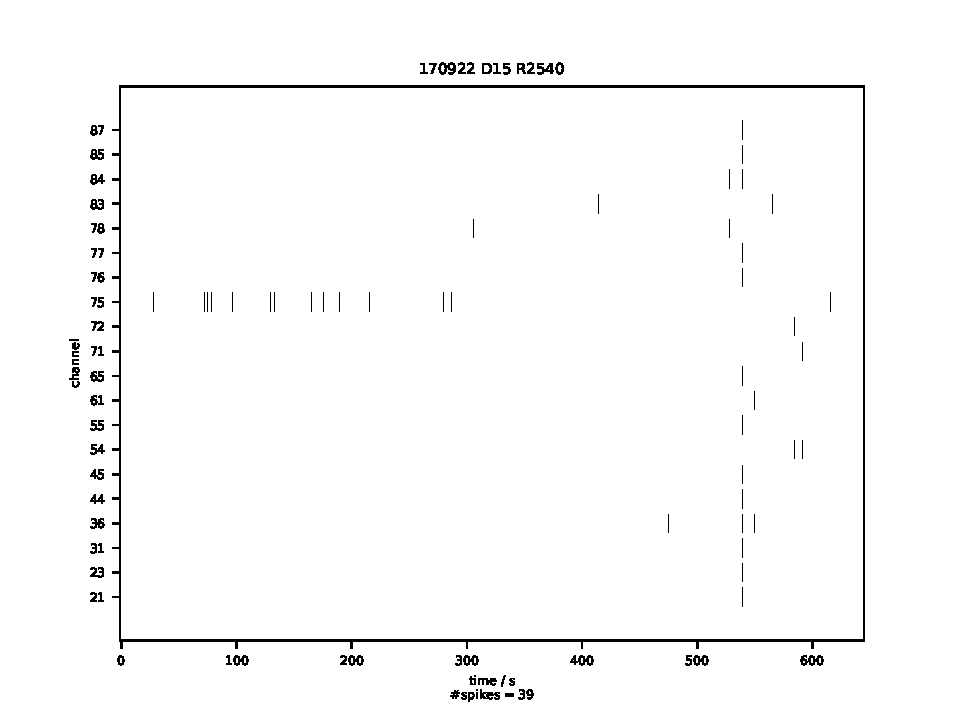
\includegraphics[width=8cm]{../plots/supplementary_figures/burst_plot_1.pdf}
  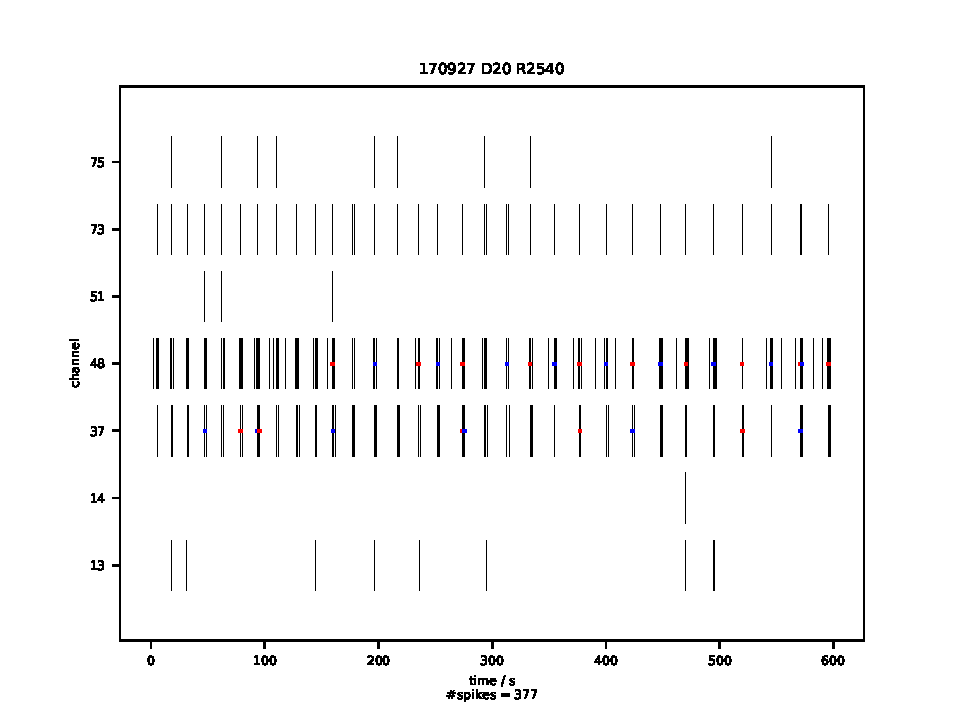
\includegraphics[width=8cm]{../plots/supplementary_figures/burst_plot_2.pdf}
  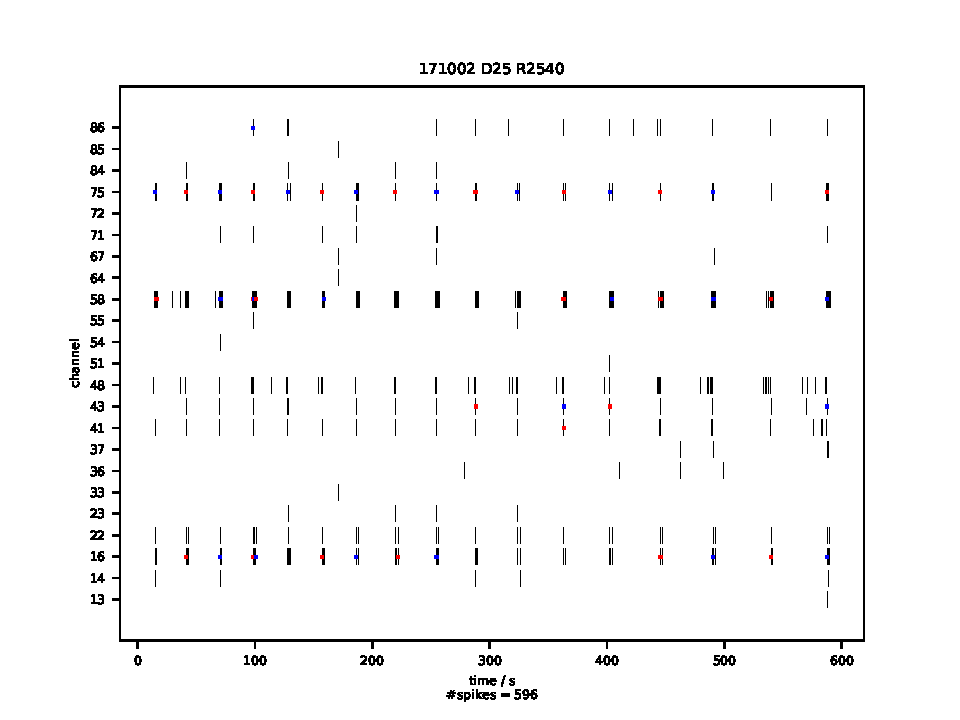
\includegraphics[width=8cm]{../plots/supplementary_figures/burst_plot_3.pdf}
  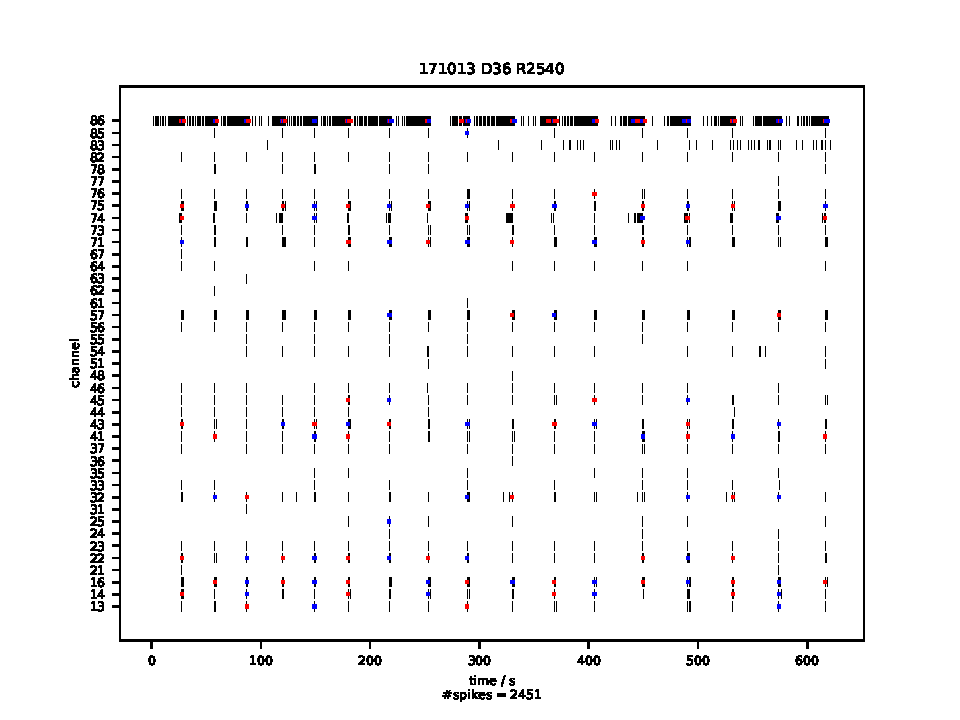
\includegraphics[width=8cm]{../plots/supplementary_figures/burst_plot_4.pdf}
  \caption{Emergence of spontaneous activity.  Show a few example rasters.
    at different developmental stages.  Perhaps show four at different
  ages in a 2x2 layout.  Or three in a 3x1 layout?}
  \label{fig:rasters}
\end{figure}


\begin{figure}
	\centering
\begin{subfigure}[b]{0.45\textwidth}
	\centering
	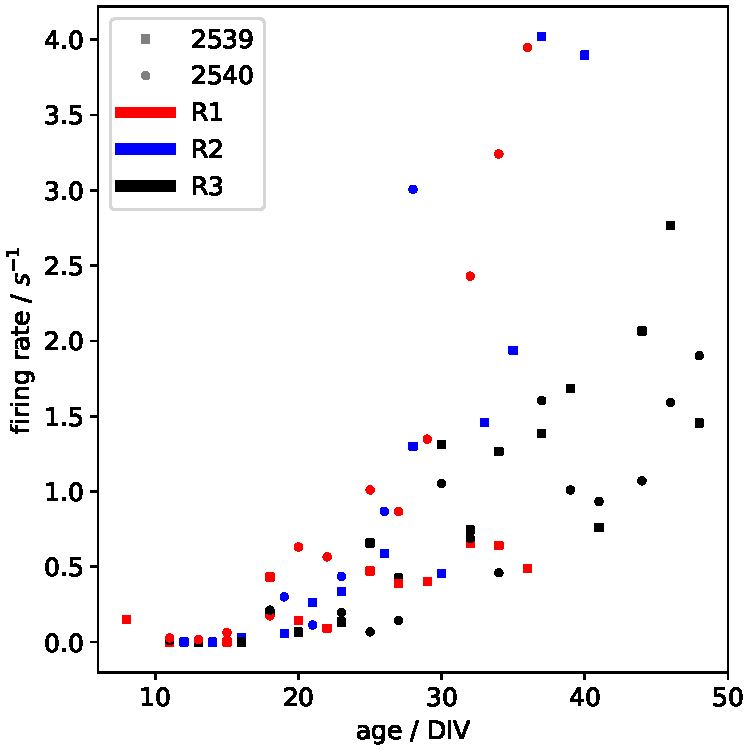
\includegraphics[width=\textwidth]{../plots/development_plots_fr.pdf}
\end{subfigure}
\hfill
\begin{subfigure}[b]{0.45\textwidth}
	\centering
	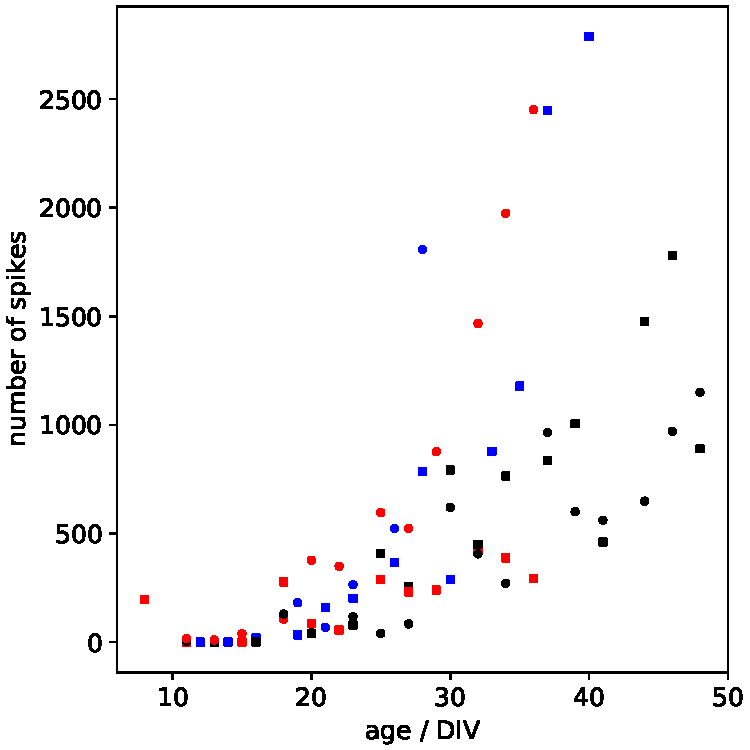
\includegraphics[width=\textwidth]{../plots/development_plots_n.pdf}
\end{subfigure}

\begin{subfigure}[b]{0.45\textwidth}
	\centering
	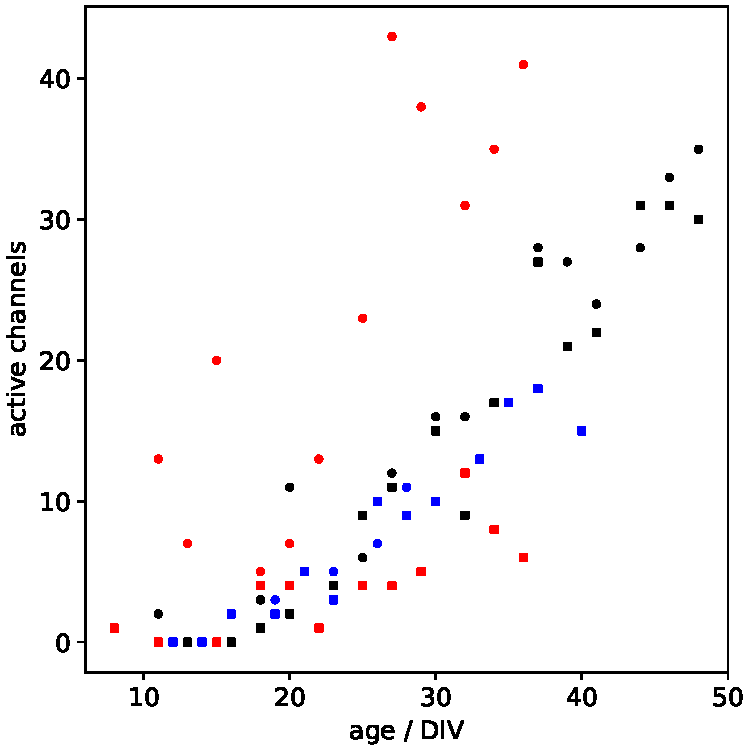
\includegraphics[width=\textwidth]{../plots/development_plots_channels.pdf}
\end{subfigure}
\hfill
\begin{subfigure}[b]{0.45\textwidth}
	\centering
	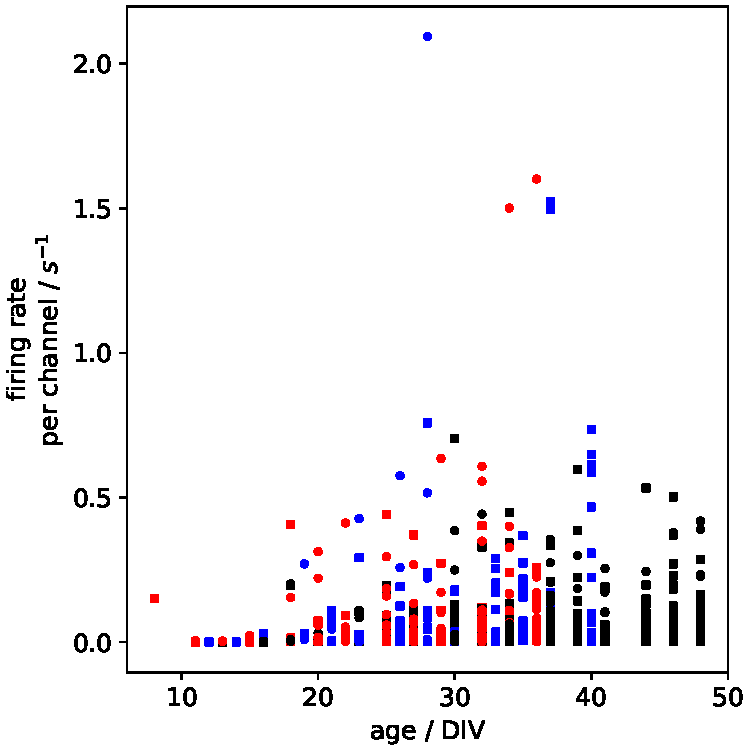
\includegraphics[width=\textwidth]{../plots/development_plots_fr_perchan.pdf}
\end{subfigure}

\begin{subfigure}[b]{0.45\textwidth}
	\centering
	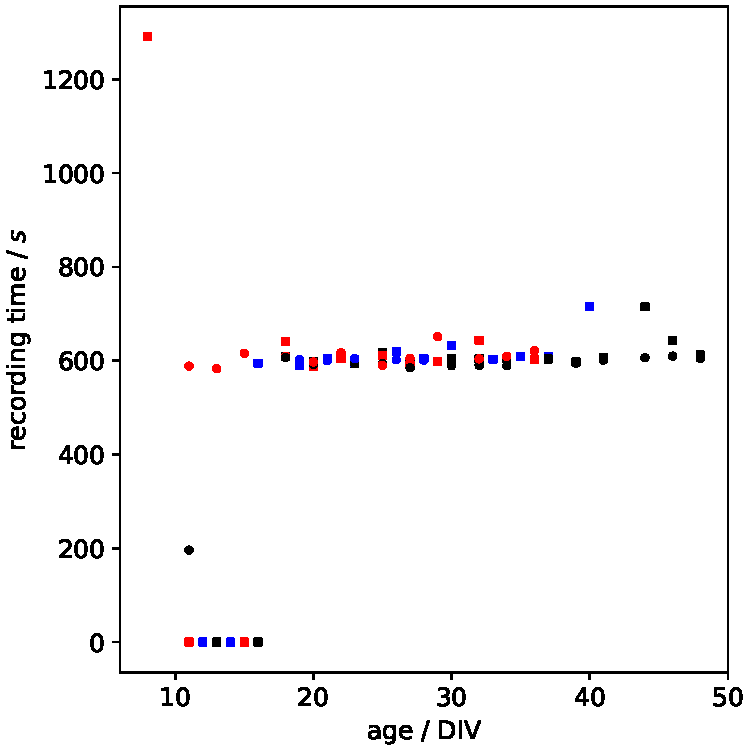
\includegraphics[width=\textwidth]{../plots/development_plots_recording_time.pdf}
\end{subfigure}

	\caption{Plots of network firing rate, number of spikes, number of active channels, recording time, and mean firing rate per channel against age. The main factor in the increase in firing rate is an increase in the number of active channels.}
	\label{fig:development}
\end{figure}


\begin{figure}
	\centering
	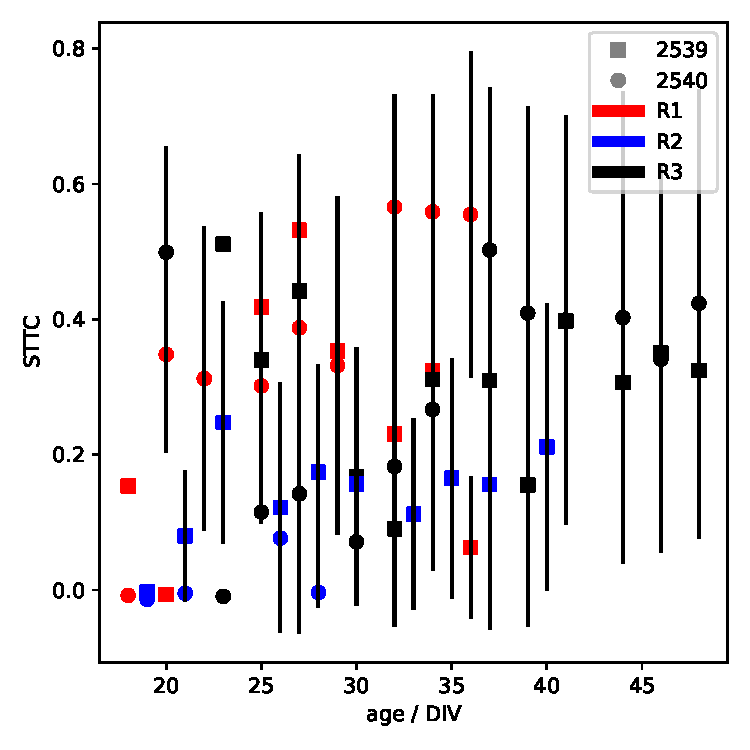
\includegraphics[width=\textwidth]{../plots/correlation_plots.pdf}
	\caption{Plots of mean STTC, calculated pairwise with a synchronicity window of 50 ms, against age. There is no discernible trend in correlation over time.}
	\label{fig:correlation}
\end{figure}


\begin{figure}
\centering
\begin{subfigure}[b]{0.7\textwidth}
	\centering
	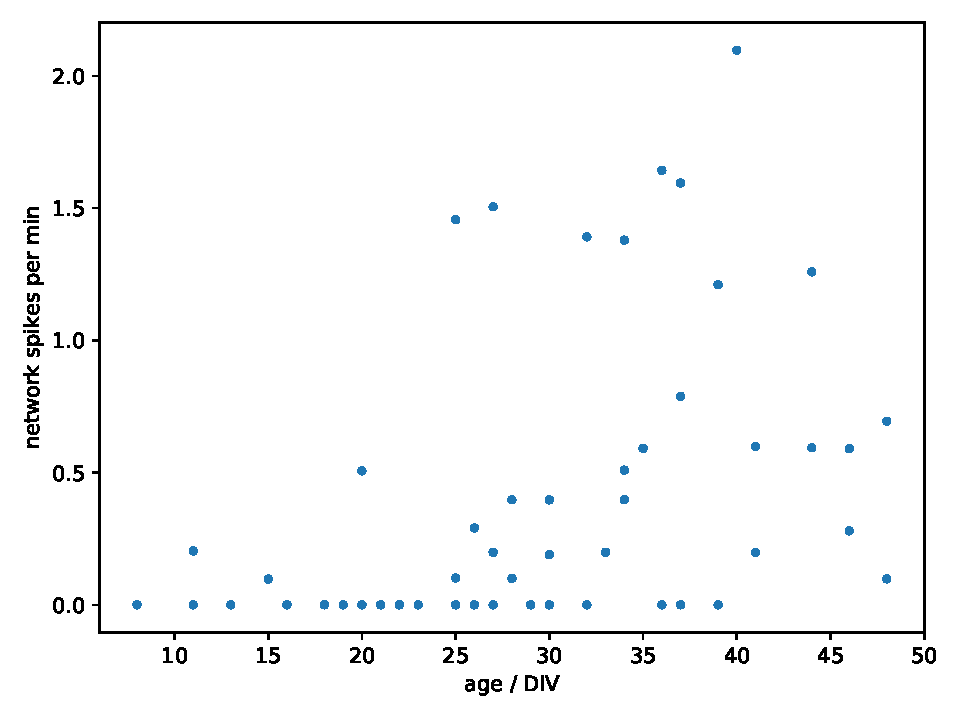
\includegraphics[width=\textwidth]{../plots/network_spikes_age.pdf}
	\caption{The rate of network spike occurrence plotted against age.}
	\label{fig:networkfreq}
\end{subfigure}

\begin{subfigure}[b]{0.7\textwidth}
	\centering
	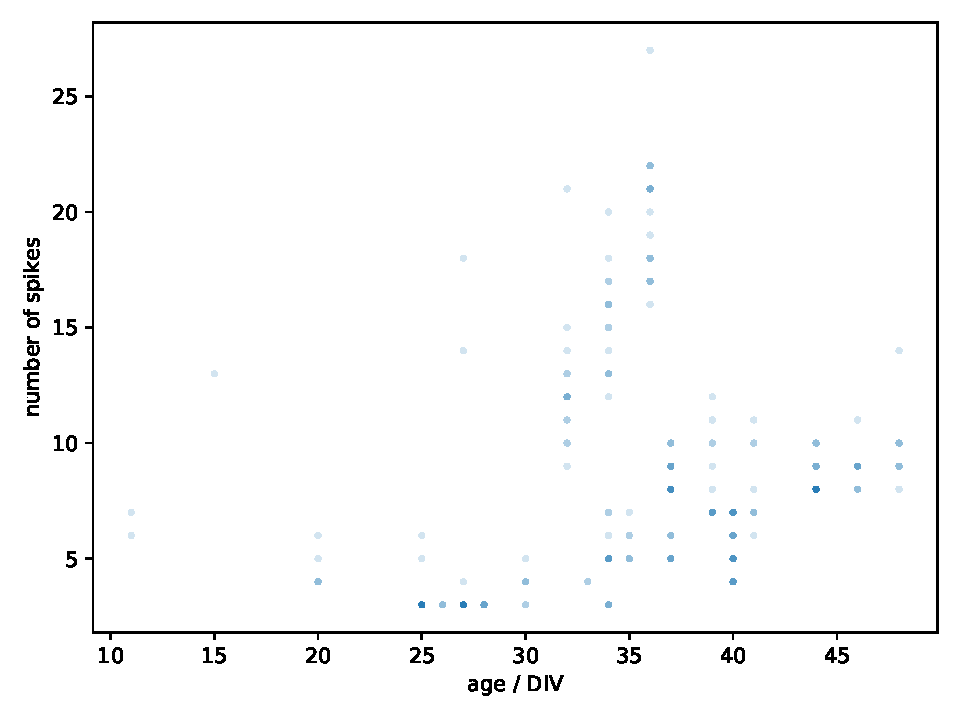
\includegraphics[width=\textwidth]{../plots/network_spikes_amplitude.pdf}
	\caption{The amplitude of network spikes plotted against age.}
	\label{fig:networkamp}
\end{subfigure}
\caption{Characteristics of network spikes.}
\end{figure}




\end{document}

%% LocalWords: Eglen MEA





